
\chapter{Algorithms and Branches\label{chpt:algorithms-and-branches}}

According to the commutativity of operations (see $\mathsection$\ref{subsec:Commutativity-between-operations}),
the only possible algorithms to evaluate $\gamma(\mathbf{r},\mathbf{\Omega})$
from $\Delta\rho(\mathbf{r},\mathbf{\Omega})$ are shown in the figure
\ref{fig:Possible-algorithms}.

\begin{figure}[h]
\begin{centering}
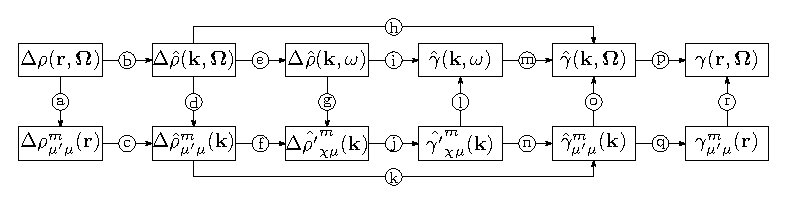
\includegraphics{_figure/algorithms}
\par\end{centering}
\caption{Possible algorithms for $\gamma$ evaluation\label{fig:Possible-algorithms}}
\end{figure}

Several branches are built to test and compare between algorithms,
which are shown below in table \ref{tab:Branch-option} and will be
detailed in the following context. \marginpar{These branches should give numerically the same result in certain
conditions, that will be discussed in later sections.}

\selectlanguage{english}%
\begin{table}[h]
\selectlanguage{american}%
\begin{centering}
\begin{tabular*}{1\textwidth}{@{\extracolsep{\fill}}cccc}
\toprule 
\tableheadline{Method} & \tableheadline{Sub-Method} & \tableheadline{Description} & \tableheadline{Theory}\tabularnewline
\midrule
reference & dipole & calculate $n(r)$ and $P(r)$ separately & $\mathsection$\ref{chpt:mdft} \textcolor{red}{{[}ref{]}}\tabularnewline
\midrule
naive & standard & use $c_{\mu\nu,\chi}^{mn}(k)$ as input DCF & $\mathsection$\ref{subsec:Using-projections-in-1}\tabularnewline
 & zero-order & use $\hat{c}(k,\boldsymbol{\omega_{1}},\boldsymbol{\omega_{2}})$
and take the nearest point & $\mathsection$\ref{subsec:Zero-order-interpolation-of}\tabularnewline
 & interpolation & use $\hat{c}(k,\boldsymbol{\omega_{1}},\boldsymbol{\omega_{2}})$
with linear interpolation  & $\mathsection$\ref{subsec:Linear-interpolation-of}\tabularnewline
 & dipole & use $c_{S}$, $c_{\Delta}$, $c_{D}$ issue from \textcolor{red}{{[}ref{]}} & $\mathsection$\ref{subsec:Using-projections-in}\tabularnewline
 & nmax1 & use $c_{S}$, $c_{\Delta}$, $c_{D}$, $c_{\pm}$ issue from {\footnotesize{}\citep{puibasset_bridge_2012}} & $\mathsection$\ref{subsec:Using-projections-in}\tabularnewline
\midrule
convolution & standard & algorithm with symmetry reduction & $\mathsection$\ref{subsec:Reduction-by-symmetry}\tabularnewline
 & asymm  & algorithm without symmetry reduction & $\mathsection$\ref{subsec:Reduction-by-symmetry}\tabularnewline
 & pure\_angular  & inverse FFT and FGSHT & $\mathsection$\ref{chpt:algorithms-and-branches}\tabularnewline
\bottomrule
\end{tabular*}
\par\end{centering}
\selectlanguage{english}%
\caption{\foreignlanguage{american}{Branch option in MDFT\label{tab:Branch-option}}}
\end{table}

\selectlanguage{american}%

\section{Branches \textquotedbl{}naive\textquotedbl{} }

Branches \texttt{\textbf{naive}} are the algorithms mentioned in section
\ref{chpt:fft-spatial}, which go through the path 
\[
\left(b\right)\shortrightarrow\left(h\right)\shortrightarrow\left(p\right)
\]
 in figure \ref{fig:Possible-algorithms}, calculating directly $\hat{\gamma}(\mathbf{k},\mathbf{\Omega})$
from $\Delta\hat{\rho}(\mathbf{k},\mathbf{\Omega})$. The difference
between branches is the way to calculate $\hat{c}(\mathbf{k},\mathbf{\Omega_{1}},\mathbf{\Omega_{2}})$.
Branch\textbf{ }\texttt{\textbf{naive\_standard}} use $c_{\mu\nu,\chi}^{mn}(k)$
as input \acs{DCF}. Branch \texttt{\textbf{naive\_zero-order}} and
\texttt{\textbf{naive\_interpolation}} using $\hat{c}(k,\boldsymbol{\omega_{1}},\boldsymbol{\omega_{2}})$
with zero-order and linear interpolation, where the former is rejected
in the implementation due to a lack of precision (appendix \ref{chpt:error-evaluation-interpolation-DCF}).

\section{Branches \textquotedbl{}convolution\textquotedbl{}}

Branches\textbf{ }\texttt{\textbf{convolution\_asymm}} and \texttt{\textbf{convolution\_standard}}
are operational algorithms of angular convolution show in section
\ref{chpt:angular-convolution}, which go through the path 
\[
\left(a\right)\shortrightarrow\left(c\right)\shortrightarrow\left(f\right)\shortrightarrow\left(j\right)\shortrightarrow\left(n\right)\shortrightarrow\left(q\right)\shortrightarrow\left(r\right)
\]

Branches\textbf{ }\texttt{\textbf{convolution\_asymm}} uses the original
operational algorithm ($\mathsection$\ref{sec:Operational-algorithm})
without symmetry reduction ($\mathsection$\ref{subsec:Reduction-by-symmetry}),
and \texttt{\textbf{convolution\_standard}} with it. 

Branch \texttt{\textbf{convolution\_pure\_angular}} goes through the
path 
\[
\left(b\right)\shortrightarrow\left(d\right)\shortrightarrow\left(f\right)\shortrightarrow\left(j\right)\shortrightarrow\left(n\right)\shortrightarrow\left(o\right)\shortrightarrow\left(p\right)
\]
which inverse the first and last two steps of the two algorithms mentioned
above.

\section{Testing branches for $n_{\max}$=1}

Branches \texttt{\textbf{naive\_dipole}}, \texttt{\textbf{naive\_nmax1}}
pass by $\left(b\right)\shortrightarrow\left(h\right)\shortrightarrow\left(p\right)$
, using DCF separately of the references \textcolor{red}{{[}ref{]}}
and {\footnotesize{}\citep{puibasset_bridge_2012}}, whose slight
difference is shown in $\mathsection$\ref{subsec:Comparison-with-non-coupling}.
Branch \texttt{\textbf{reference\_dipole}} use DCF in \textcolor{red}{{[}ref{]}},
which is the original method in MDFT to calculate $\mathcal{F}_{\mathrm{exc}}$
via multipole expansion. In addition with branch \texttt{\textbf{convolution\_standard}},
which can also use the two DCF mentioned above, a test of validation
can be performed, which should at any case exactly numerically the
same if the same DCF is used.

\section{Other paths}

Considering the necessity, other paths such as those passing by $\left(i\right)$
and $\left(k\right)$ are only built for local test usage (c. f. discussion
in following sections).
